\documentclass{article} % For LaTeX2e
\usepackage{nips_adapted,times}
\usepackage{hyperref}
\usepackage{url}
\usepackage{amssymb}
\usepackage{amsmath}
\usepackage{graphicx}
\usepackage{subfig}

\title{Multivariate Optimization for Non-decomposable Performance Measure}


\author{
Debojyoti Dey \\
15511264 \\
\And
Nimisha Agarwal \\
15511267 \\
}

% The \author macro works with any number of authors. There are two commands
% used to separate the names and addresses of multiple authors: \And and \AND.
%
% Using \And between authors leaves it to \LaTeX{} to determine where to break
% the lines. Using \AND forces a linebreak at that point. So, if \LaTeX{}
% puts 3 of 4 authors names on the first line, and the last on the second
% line, try using \AND instead of \And before the third author name.

\newcommand{\fix}{\marginpar{FIX}}
\newcommand{\new}{\marginpar{NEW}}

\nipsfinalcopy

\begin{document}


\maketitle

\section{Problem Statement}

The goal of the project is to find a general optimization technique to maximize performance measures which are non-decomposable in nature. These are application specific measures and cannot be expressed as a sum of losses on individual data points. One such performance metric is \textit{F-Measure}, expressed as a function of True Positive Rate(TPR) and True Negative Rate(TNR) and often used in class imbalanced classification settings. Another example of non-decomposable performance measure is \textit{precision@k} used in ranking problem where true positiveness of top $k$ elements are to be evaluated. \textit{AUC} is used to compute the area under ROC curve in order to minimize the number of wrongly ordered instances in ranking problem. \textit{pAUC}(partial AUC) is used to limit this evaluation within the region of top-ranked elements. This is the fact that keeps such optimization problems from participating directly in standard batch or online setting of gradient based optimization techniques.

The need for non-additive performance measure derived from the whole sample arises because of the limitation of loss function such as misclassification rate, as it simply predicts the majority class which fails to predict correctly for the instances belonging to minority class in class imbalanced settings. Examples of non-decomposable performance measures include F-measure, G-mean, H-mean etc.

Several efforts have been made to solve optimization problems with non-decomposable performance measures. They can be broadly categorized into 1) surrogate based approach which tries to minimize hinge loss as an upper bound to binary misclassification in multivariate settings. Cutting plane learning with structural SVM \cite{c1} reduces the problem of minimizing non-decomposable loss to multivariate optimization. 2) Probabilistic plug-in classifier\cite{c3} model tries to find class probability estimator empirically from the training set and maximize the performance measure by obtaining a suitable threshold from test set. 3) Cost-sensitive classification based approach\cite{c6} maximizing performance measure in the form of pseudo linear function on TPR and TNR such as \textit{F-measure}. 4) Stochastic primal dual solver(SPADE)\cite{c2} constructs dual of concave performance measure functions like G-mean, H-mean and performs gradient ascent and gradient descent over primal and dual space respectively. It gives convergence guarantee for loss functions with bounded gradient. Stochastic Alternate Maximization(STAMP)\cite{c2} procedure tries to maximize pseudo linear performance measure in terms of TPR and TNR. \textit{F-measure} is one such candidate eligible for such optimization.

Though there exist stochastic gradient methods such as \textbf{SPADE} which can maximize non-decomposable loss in online fashion\cite{c2} as mentioned above, such methods assume gradient of the loss function to be bounded. Our attempt in this work is to alleviate such restriction and propose a generic model to maximize concave loss function including the ones having large gradient such as that of G-mean.


\section{Multivariate Optmization Setting}
The learning problem tries to find a mapping from input vector $x \in \mathcal{X}$ to the label $y \in \mathcal{Y}$. We consider our training samples $(x_1,y_1),\ldots,(x_n,y_n) \in \mathcal{X} \times \mathcal{Y}$ drawn $\textit{iid}$ from some unknown underlying distribution $\mathcal{D}$. We are concerned with binary classification with $\mathcal{X} \subseteq \mathbb{R}^d$ and $\mathcal{Y}=\{-1,+1\}$. The goal is to find rule $h \in \mathcal{H}$ from hypothesis space $\mathcal{H}$ such that it optimizes the expected prediction performance over $S \in (\mathcal{X} \times \mathcal{Y})^n$. The prediction performance is defined as the following,
$$
R^{\Delta}(h) = \int \Delta((h(x_1),\ldots,h(x_n)),(y_1,\ldots,y_n))dPr(S)
$$
If the loss function $\Delta$ decomposes into sum of individual loss function $\delta$ of each example then the following holds,
$$
\Delta((h(x_1),\ldots,h(x_n)),(y_1,\ldots,y_n)) = \frac{1}{n} \sum\limits_{i=1}^{n}\delta(h(x_i),y_i)
$$
Since examples are $iid$, the equation can be simplified to,
$$
R^{\Delta}(h) = R^{\delta}(h) = \int\limits_{\mathcal{X}\times\mathcal{Y}}\delta(h(x),y)dPr(x,y)$$
Discriminative learning approximate this loss function over empirical risk $R^{\delta}_{S}(h)$, that is over the training set $S$ given by,
$$
\hat{R}^{\delta}_{S}(h) = \frac{1}{n}\sum\limits_{i=1}^{n}\delta(h(x_i),y_i)
$$
Thus a learning problem with decomposable performance measure can be solved by any discriminative learning algorithm which optimizes uni variate loss function defined over individual training instances. However, non-decomposable loss function cannot be broken down to individual example level. As an example, generalized F-measure with the following form,
$$
F_\beta = (1+\beta^2) \frac{precision . recall}{\beta^2 . precision + recall}
$$
for any particular $h$. Such performance measure over the entire training set $S$ cannot be expressed as sum of point-wise performance measure $\delta$. Hence we need to optimize the empirical loss function $\Delta$ over the entire sample set.
$$
\hat{R}^{\Delta}_{S}(h)=\Delta((h(x_1),\ldots,h(x_n)),(y_1,\ldots,y_n))
$$
We realise that the complexity of the prediction algorithm becomes exponential due to the size of the label search space. Each possible assignment of labels $\{y_i\}_1^n$ contributes to a constraint we will see in optimization problem giving exponential dimensional constraint space. Multivariate optimization technique such as structural SVM incrementally builds the constraint space and thus gives a tractable solution.

\section{Structural SVM}

Struct SVM used for multi-class classification.
\begin{equation*}
\begin{split}
& \underset{w,\xi \geq 0}{min} \quad \frac{1}{2}\|w\|^2+C\xi\\
& s.t \quad \forall\overline{y} \in \overline{\mathcal{Y}}\setminus\overline{y}^*:w^T[\psi(\overline{x},\overline{y}^*)- \psi(\overline{x},\overline{y})]\geq \Delta(\overline{y}^*,\overline{y})-\xi\\
& \Rightarrow \Delta(\overline{y}^*,\overline{y}) + \Sigma (y_i - y_i^*)w^Tx_i \leq \xi
\end{split}
\end{equation*}
where $\Delta(\overline{y}^*,\overline{y})$ is loss function.	
$\xi$ is the upper bound of loss function.
We substitute margin violation $\xi$ in objective function by
\begin{align}
\label{eqn:1}
\mathcal L_w(\overline{x},\overline{y}^*)=\max_{\overline{y}\in\{1,-1\}^n}\{\Delta(\overline{y}^*,\overline{y}) + \sum_{i=1}^n (y_i - y_i^*)w^Tx_i\}
\end{align}

\section{Formulation of Optimization problem}
We work with concave performance measure which is a function of True positive rate(TPR) and True negative rate(TNR) as following:
$$
\mathcal{P}_w = \Psi(P(w),N(w))
$$
where $P(w)$ and $N(w)$ represent TPR and TNR corresponding to the classifier given by $w$. 
Performance measure G-mean is given by
\begin{align*}
\phi(P,N) &=\sqrt{PN}\\
& = \min_{\alpha,\beta}\{\alpha P+\beta N - \phi^*(\alpha,\beta)\}
\end{align*}
as $\phi$ is a concave function. P,N stands for TPR and TNR respectively. We define our loss function as
\begin{align*}
\Delta(\overline{y}^*,\overline{y}) &= -\phi(P,N) \\
&= \max_{\alpha,\beta}\{-\alpha P-\beta N + \phi^*(\alpha,\beta)\}\\
%		&= \max_{\alpha,\beta}\{\alpha P+\beta N - (-\phi^*(-\alpha,-\beta))\}
\end{align*}
We can re-write equation \ref{eqn:1} as,
\begin{align}
\label{eqn:2}
&\mathcal L_w(\overline{x},\overline{y}^*)\nonumber\\
&=\max_{\overline{y}\in\{1,-1\}^n}\{\max_{\alpha,\beta}\{-\alpha P-\beta N +\phi^*(\alpha,\beta)\} + \frac{1}{n}\sum_{i=1}^n (y_i - y_i^*)w^Tx_i\}\nonumber\\
&=\max_{\alpha,\beta}\{\max_{\overline{y}}\{-\alpha P-\beta N  + \frac{1}{n}\sum_{i=1}^n (y_i - y_i^*)w^Tx_i\}+\phi^*(\alpha,\beta)\}
\end{align}
We use the notations $y_i^{\star}$ and $y_i$ respectively representing the given and predicted label for $i^{th}$ training instance. $y_i^{\star},y_i\in\mathcal{Y}$, where $\mathcal{Y}=\{-1,+1\}$. TPR and TNR can be represented as the following:
\begin{align*}
&P = \sum_{i=1}^nP_i(y_i,y_i^*)= \frac{1}{n_+}\sum_{i=1}^n\frac{(1+y_i)(1+y_i^*)}{4}\\
&N = \sum_{i=1}^nN_i(y_i,y_i^*)= \frac{1}{n_-}\sum_{i=1}^n\frac{(1-y_i)(1-y_i^*)}{4}
\end{align*}
We are interested in the dual representation of multivariate loss function as below. 
\begin{equation}
\begin{split}
\Delta(\overline{y}^\star,\overline{y}) & = -\mathcal{P}_w = -\Psi(P(w),N(w))\\
& = -\inf_{\alpha,\beta}\{\alpha P(w)+\beta N(W)-\Psi^\star(P(w),N(w))\}\\
& = \sup_{\alpha,\beta}\{-\alpha P(w)-\beta N(W)+\Psi^\star(P(w),N(w))\}
\end{split}
\end{equation}
Substituting, inner maximization becomes,
\begin{equation}
\sum_{i=1}^n\max_{y_i\in\{-1,+1\}}-\frac{\alpha}{n_+}\frac{(1+y_i)(1+y_i^*)}{4} - \frac{\beta}{n_-}\frac{(1-y_i)(1-y_i^*)}{4} + \frac{1}{n}(y_i - y_i^*)w^Tx_i
\end{equation}
This enables point-wise optimization. Once we solve the inner maximization problem, the outer maximization can be solved using \textbf{SPADE}\cite{c2}, using the primal dual gradient method. Now we need to solve the inner maximization problem. Our hope is to reduce the inner optimization problem to weighted hinge loss which can easily be solved by weighted SVM solver.

Solving the above maximization, we get the following weighted hinge loss like function with some additional constants,
\begin{align*}
\sum_{i=1}^n
(\frac{\alpha}{n_+}\max\{0,1-y_i^*\frac{2n_+}{\alpha n}w^Tx_i\}
- \frac{\alpha}{n_+})\mathbb{I}(y^*_i=1)\\
+ (\frac{\beta}{n_-}\max\{0,1-y_i^*\frac{2n_-}{\beta n}w^Tx_i\}
- \frac{\beta}{n_-})\mathbb{I}(y^*_i=-1)
\end{align*}
Now we can re-write equation \ref{eqn:2} as following
\begin{align*}
\mathcal L_w(\overline{x},\overline{y}^*) = \max_{\alpha,\beta}\{
\frac{\alpha}{n_+}\sum_{y_i^*=1}\max\{0,1-y_i^*\frac{2n_+}{\alpha n}w^Tx_i\}+\frac{\beta}{n_-}\sum_{y_i^*=-1}\max\{0,1-y_i^*\frac{2n_-}{\beta n}w^Tx_i\}-(\alpha+\beta)+\phi^*(\alpha,\beta)\}
\end{align*}

We can substitute the loss in struct SVM to get the final objective function:
\begin{align*}
\min_w \frac{||w||^2}{2} + & C \mathcal L_w(\overline{x},\overline{y}^*)\\
&\equiv \min_w \frac{||w||^2}{2} + C\max_{\alpha,\beta}\{
\frac{\alpha}{n_+}\sum_{y_i^*=1}\max\{0,1-y_i^*\frac{2n_+}{\alpha n}w^Tx_i\}\\
&+ \frac{\beta}{n_-}\sum_{y_i^*=-1}\max\{0,1-y_i^*\frac{2n_-}{\beta n}w^Tx_i\}\\
&-(\alpha+\beta)+\phi^*(\alpha,\beta)\}
\end{align*}

\begin{figure}
\subfloat[Change of True positive(negative) rate]{
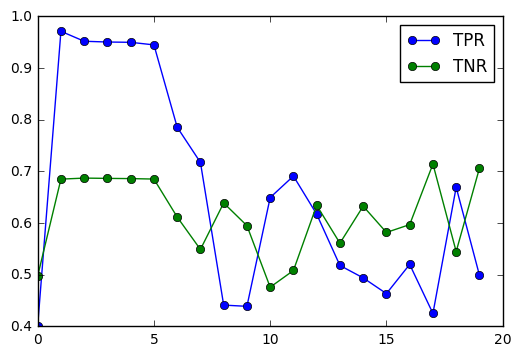
\includegraphics[scale=0.55]{pix/plot_ijcnn.png}
}
\subfloat[Change of G-mean]{
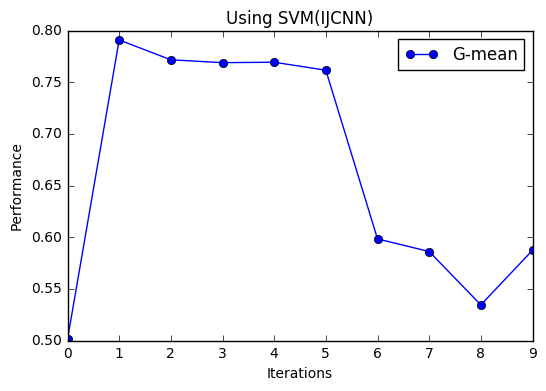
\includegraphics[scale=0.55]{pix/gmean_ijcnn.png}
}
\caption{Accuracy variation for IJCNN data, X-axis represents iteration}
\label{fig:acc_ijcnn}
\end{figure}

\section{Experimental Result}

The above objective function has two components. The inner maximization problem is solved by gradient ascent and the outer minimization is solved by SVM. We initialize $w$ randomly. Then we perform the following steps in each iterative cycle:
\begin{enumerate}
	\item Fix $w$
	\item Gradient ascent on $\mathcal L_w(\overline{x},\overline{y}^*)$ wrt $\alpha,\beta$
	\item Fix $\alpha,\beta$
	\item Perform SVM wrt $w$
	\item Go to step 1
\end{enumerate}
In the second step, we improve the result of gradient ascent by tweaking the computation of gradient. Usually the first term of the function considered contributes $(\alpha/n_+)$ for any positive instance(similarly $(\beta/n_-)$ for negative instance) to the gradient if hinge loss margin is violated by that. In our method we only add the contribution only if the istance is misclassified i.e. on the wrong side of hyperplane. We use dynamic step length using cross-validation. In the fourth step, We use Liblinear solver to perform SVM. We use weighted hinge loss function.

We have run our experiment on two datasets, a) IJCNN and b) Covertype. We plot change of accuracy with each cycle. We have shown accuracy in terms of TPR and TNR as well as G-mean. Fig \ref{fig:acc_ijcnn} shows the variation of accuracy over the iterations for IJCNN data. Fig \ref{fig:acc_cov} shows accuracy variation for Covertype data.

\begin{figure}
\subfloat[Change of True positive(negative) rate]{
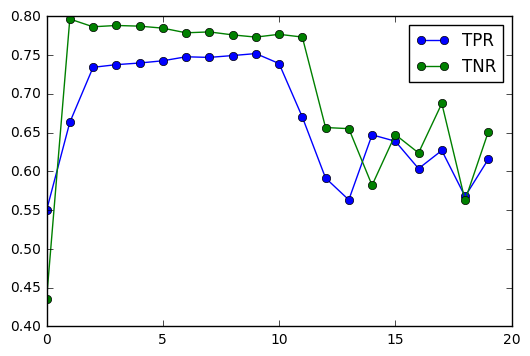
\includegraphics[scale=0.55]{pix/plot_cov.png}
}
\subfloat[Change of G-mean]{
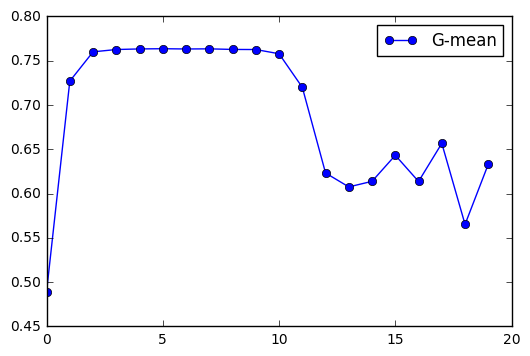
\includegraphics[scale=0.55]{pix/gmean_cov.png}
}
\caption{Accuracy variation for Covertype data, X-axis represents iteration}
\label{fig:acc_cov}
\end{figure}
\section{Conclusion}

....

\begin{thebibliography}{99}
	
	\bibitem{c1} Joachims, Thorsten. "A support vector method for multivariate performance measures." Proceedings of the 22nd international conference on Machine learning. ACM, 2005.
	\bibitem{c2} Narasimhan, Harikrishna, Purushottam Kar, and Prateek Jain. "Optimizing Non-decomposable Performance Measures: A Tale of Two Classes." 32nd International Conference on Machine Learning (ICML). 2015.
	\bibitem{c3} Narasimhan, Harikrishna, Rohit Vaish, and Shivani Agarwal. "On the statistical consistency of plug-in classifiers for non-decomposable performance measures." Advances in Neural Information Processing Systems. 2014.
	\bibitem{c4} Joachims, Thorsten, Thomas Finley, and Chun-Nam John Yu. "Cutting-plane training of structural SVMs." Machine Learning 77.1 (2009): 27-59.
	\bibitem{c5} Kar, Purushottam, Harikrishna Narasimhan, and Prateek Jain. "Online and stochastic gradient methods for non-decomposable loss functions." Advances in Neural Information Processing Systems. 2014.
	\bibitem{c6} Parambath, Shameem Puthiya, Nicolas Usunier, and Yves Grandvalet. "Optimizing F-measures by cost-sensitive classification." Advances in Neural Information Processing Systems. 2014.
	
\end{thebibliography}

\end{document}
